\section{Hosting \& Deployment}

Die prototypische Umsetzung des Quiz-Systems kann unter der folgenden URL aufgerufen werden: \textit{https://study-quiz.com}. \newline

\noindent Im folgenden Abschnitt wird das Hosting, die kontinuierliche Integration der prototypischen Entwicklung behandelt. 
Zudem werden in entsprechenden Abschnitten Unterschiede zu einer Anwendung im Produktivbetrieb erläutert.

\subsection{CI / CD}

Die Entwicklung der prototypischen Umsetzung des Quiz-Systems wurde unter Verwendung der
Source-Code-Verwaltungsplattform GitHub durchgeführt. Hierbei wurde der Quellcode der Anwendung
gespeichert, und Teammitglieder konnten gemeinsam am Source-Code arbeiten. Zur Sicherstellung
der Code-Qualität wurden Skripte entwickelt, die automatisch auf sogenannten \textit{Action-Runnern}
in GitHub ausgeführt wurden, wenn Quellcode gepusht wurde. Diese Skripte stellten sicher, dass der
gepushte Quellcode erfolgreich auf einem frisch eingerichteten System kompiliert werden konnte. \newline

\noindent Im Rahmen der kontinuierlichen Integration wurde ein Skript entwickelt, das sowohl das User-Interface 
als auch das Backend in Docker-Containern kompilierte und über die integrierte Container-Registry 
in GitHub bereitstellte. Nach jeder Implementierung eines Features durch einen Entwickler stand 
somit eine Docker-Container-Version zur Verfügung, die auf einem Testserver getestet werden konnte.

\notebox {
  Im produktiven Betrieb würde zusätzlich mit Docker-Container-Tags gearbeitet werden.
  Container, die automatisch durch einen Push auf den Master-Branch erstellt wurden, erhielten einen 
  QA-Tag (Quality Assurance). Ein Container, der über ein Release erstellt wurde, würde eine 
  offizielle Versionsnummer als Tag erhalten.\newline

  Auf diese Weise könnte ein QA-Server erstellt werden, auf dem die Docker-Container mit dem neuesten 
  QA-Tag getestet werden. Auf dem Produktivserver würden nur Container mit einer offiziellen 
  Versionsnummer ausgeführt.
}

\subsection{Deployment}

Für das deployment der prototypischen Umsetzung des Quiz-Systems wurde ein Server bei \textit{Ionos} 
gemietet. Auf diesem Server wurde Docker installiert, um die Container, die im Rahmen der
kontinuierlichen Integration erstellt wurden, auszuführen.\newline

\noindent Die Container wurden über die integrierte Container-Registry in GitHub bereitgestellt.
Diese Container werden in einer Docker-Compose Datei definiert, die auf dem Server ausgeführt wird.
Diese Docker-Compose Datei enthält die Container für das User-Interface, das Backend und die Datenbank.
Außerdem enthält sie noch einen Webserver, welcher die Anfragen an den richtigen Cotnainer weitergeleitet.\newline

\noindent Die Container werden über die Docker-Compose Datei gestartet, indem die Datei auf dem Server
heruntergeladen wird und anschließend der Befehl \textit{docker-compose up} ausgeführt wird. \\

\begin{figure}[H]
  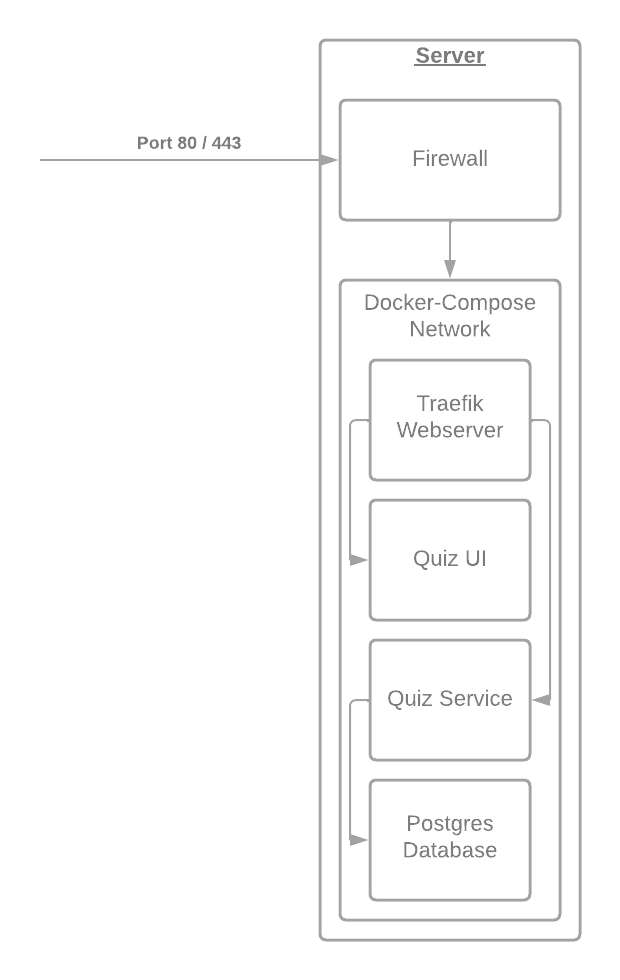
\includegraphics[width=\linewidth]{img/Hosting.png}
  \caption{Deployment}
  \label{fig:deployment}
\end{figure}

\noindent Wie in der Grafik zu sehen ist auf dem Server eine Firewall installiert, die nur die Ports 80 und 443
freigibt. Über diese Ports werden die Anfragen an den Webserver Traefik weitergeleitet, welcher sich auch
in einem Docker Container befindet. Dieser Webserver hat die Aufgabe den eingehenden Anfragen die richtigen
Container zuzuweisen. Außerdem sorgt dieser Webserver für eine verschlüsselte verbindung, 
indem es ein SSL-Zertifikat zu Verfügung stellt.\newline

\notebox {
  Bei einem Produktivumsetzung würde die Anwendung nicht über Docker-Compose deployed werden.
  Stattdessen würde ein Kubernetes-Cluster aufgesetzt werden, in dem die Container ausgeführt werden.
  Dies hätte den Vorteil, dass die Container automatisch neu gestartet werden, wenn sie abstürzen.
  Außerdem könnte die Anwendung über mehrere Server verteilt werden, um die Last zu verteilen.
  Das deployment auf Cubernetes-Cluster ist jedoch deutlich komplexer als das deployment über Docker-Compose.
}
